\documentclass[twocolumn, a4paper]{Zemiresume}
\usepackage[dvipdfmx]{graphicx}
\usepackage{graphicx}
\usepackage{amsmath}
\usepackage{txfonts}

%追加したパッケージ
\usepackage{siunitx}
\usepackage{xcolor}
\usepackage{url}
\usepackage{silence}
\WarningFilter{caption}{Unknown document class (or package)} % captionに関する警告を無視
\usepackage{subcaption}

\title{新人セミナー Git,Tex,ベクター画像 }
\date{2024 年 4月 12日}
%\date{2023 年 9月 1日}
\author{伊藤}
\headtitle{2025年度 新人セミナー Git,Tex,ベクター画像 Texについて}

\begin{document}
\maketitle

\section{はじめに}
ゼミ合宿ではこのpdfを参考に作成するといい感じになります.sample.texで出力確認を行い,template.texに自分の記事を書いてください.

%----------------------------------------------------------------------------------------------------------
\section{書式}
\textbf{日本語の論文では句読点は全角のカンマ「,」とピリオド「.」になる.}

windowの場合,設定の 時刻と言語 $>>$ 言語と地域 $>>$ Microsoft IME $>>$ 全般 の「句読点」「,.」(上から2番目)を選択で設定可能

%----------------------------------------------------------------------------------------------------------
\section{数値と単位}
\verb|\usepackage{siunitx}|を使用するとシンプルな記述が可能.

\begin{itemize}
  \item \SI{2}{mm}と書きたい場合は\verb|\SI{2}{mm}|と書く.
  \item A\,[\si{mm}]と書きたい場合は\verb|A\,[\si{mm}]|と書く.\verb|\SI{A}{[mm]}|と書くとエラーになる.
  \item \verb|\degree|と\verb|\degreeCelsius|を単位に使える.それぞれ\SI{5}{\degree},\SI{25}{\degreeCelsius}となる.
  \item その他詳しいことは以下のサイトを参考に\\
  {\footnotesize
    \url{http://www.yamamo10.jp/yamamoto/comp/latex/make_doc/unit/index.php}}
\end{itemize}
%----------------------------------------------------------------------------------------------------------
\section{変数の立体・斜体の使い分け}
変数の名称は文字を当てはめているだけなら斜体,意味のある名前は立体にする.
\begin{itemize}
  \item $x_\mathrm{ref}$のrefはreferenceで意味のある名前なので立体.書き方は\verb|$x_\mathrm{ref}$|
  \item 「i番目」の意味なら\verb|x_i|,入力(input)の意味なら\verb|x_\mathrm{i}|と書く.
\end{itemize}
%----------------------------------------------------------------------------------------------------------
\section{図表}
図表は図\ref{fig:ダミー図}のようにカラムの上\verb|[t]|または下\verb|[b]|に配置するとスペースが節約できる.結構馬鹿にならない.
\textbf{図表は必ず文中で引用する.}また,図番号と引用順は揃え,ぶち抜きの図の場合などどうしようもない場合を除いて引用$\rightarrow$ 図の順の方がいい.
また,図\ref{fig:画像は1つにまとめる}のように1つの画像にできるだけ情報を詰め込むようにするとよい図になる.

\begin{figure}[t]
  \centering
  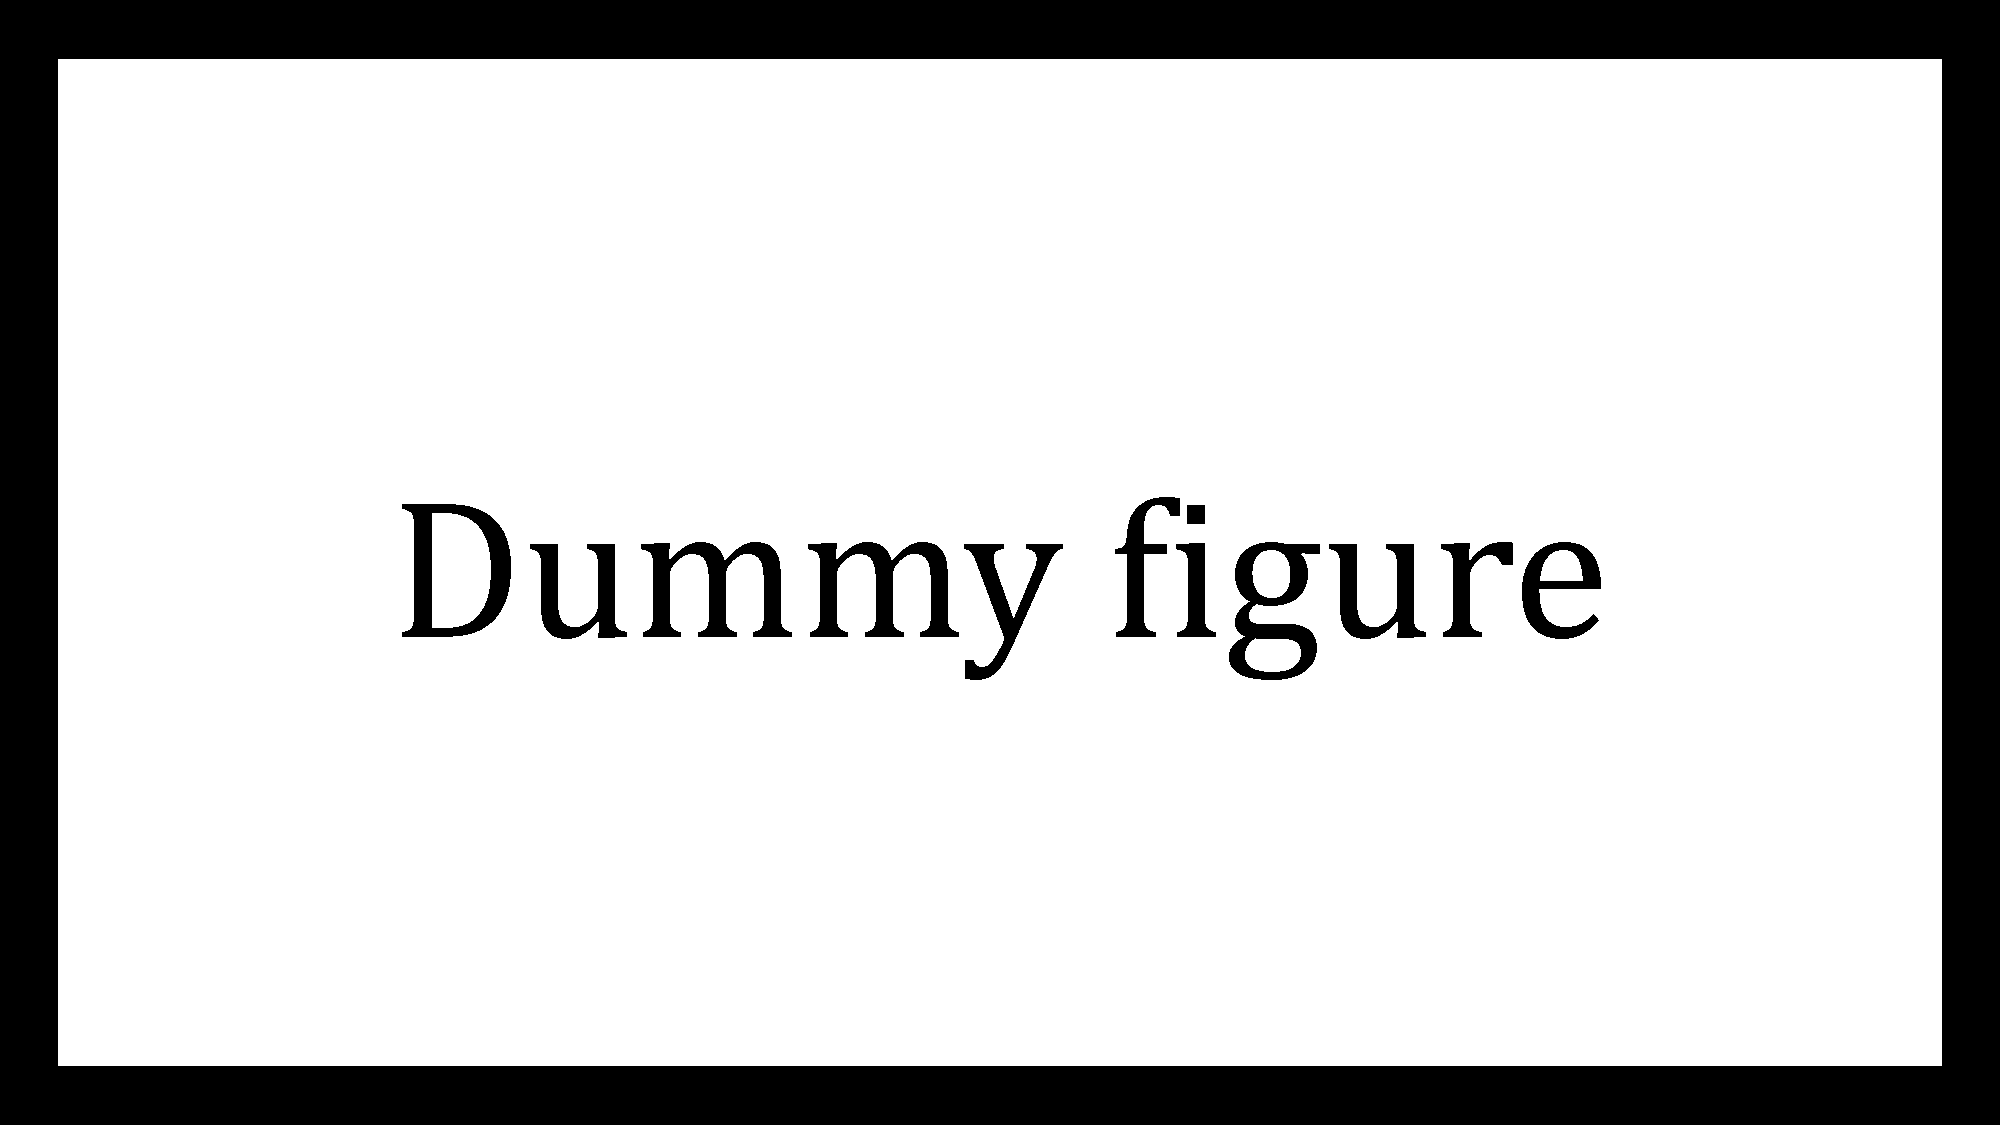
\includegraphics[width=\columnwidth]{img/Dummy.pdf}
  \caption{ダミー図}\label{fig:ダミー図}
\end{figure}
\begin{figure}[t]
  \centering
  \begin{minipage}{0.5\columnwidth}
    \centering
    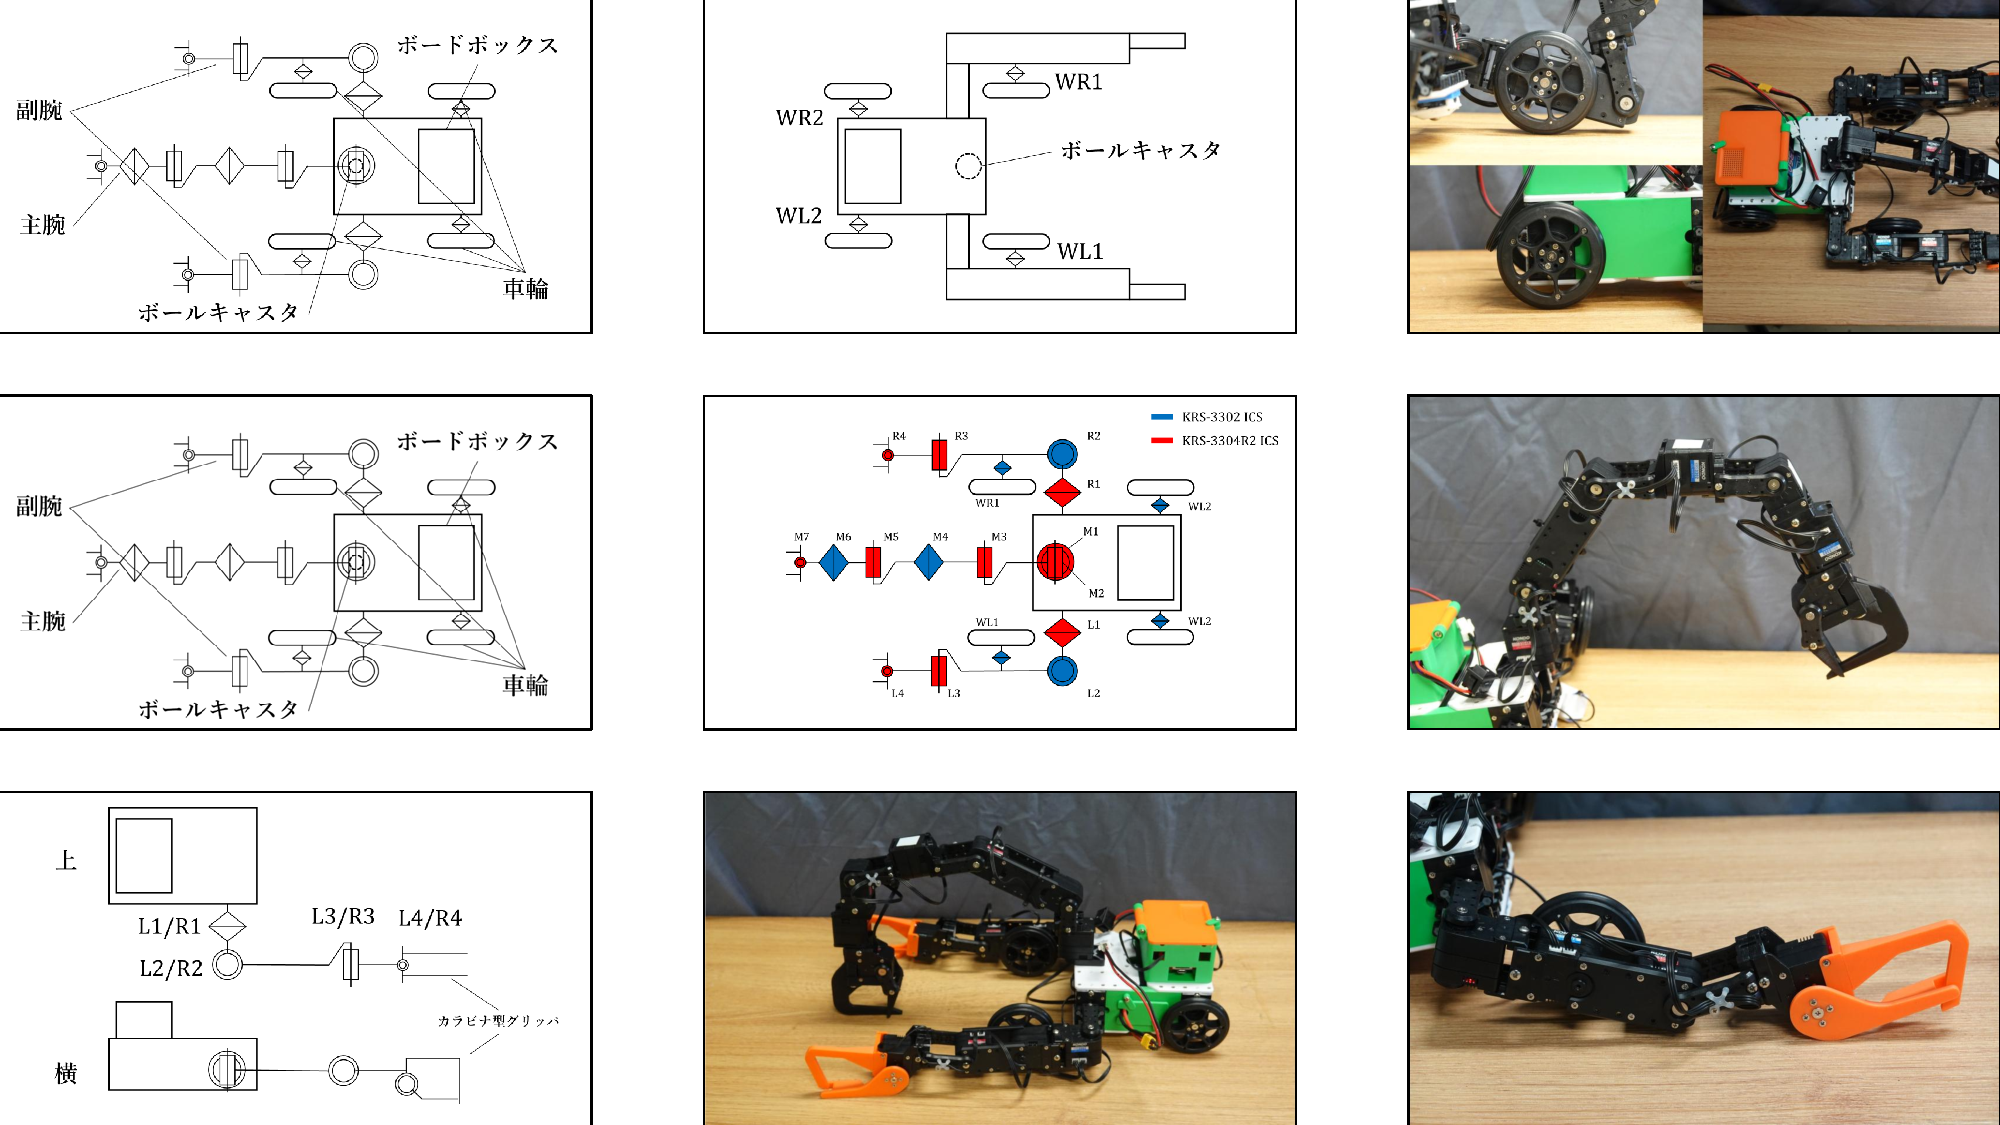
\includegraphics[width=.98\linewidth]{img/画像の集約_悪い例.pdf}
    \subcaption{悪い例}
  \end{minipage}%
  \begin{minipage}{0.5\columnwidth}
    \centering
    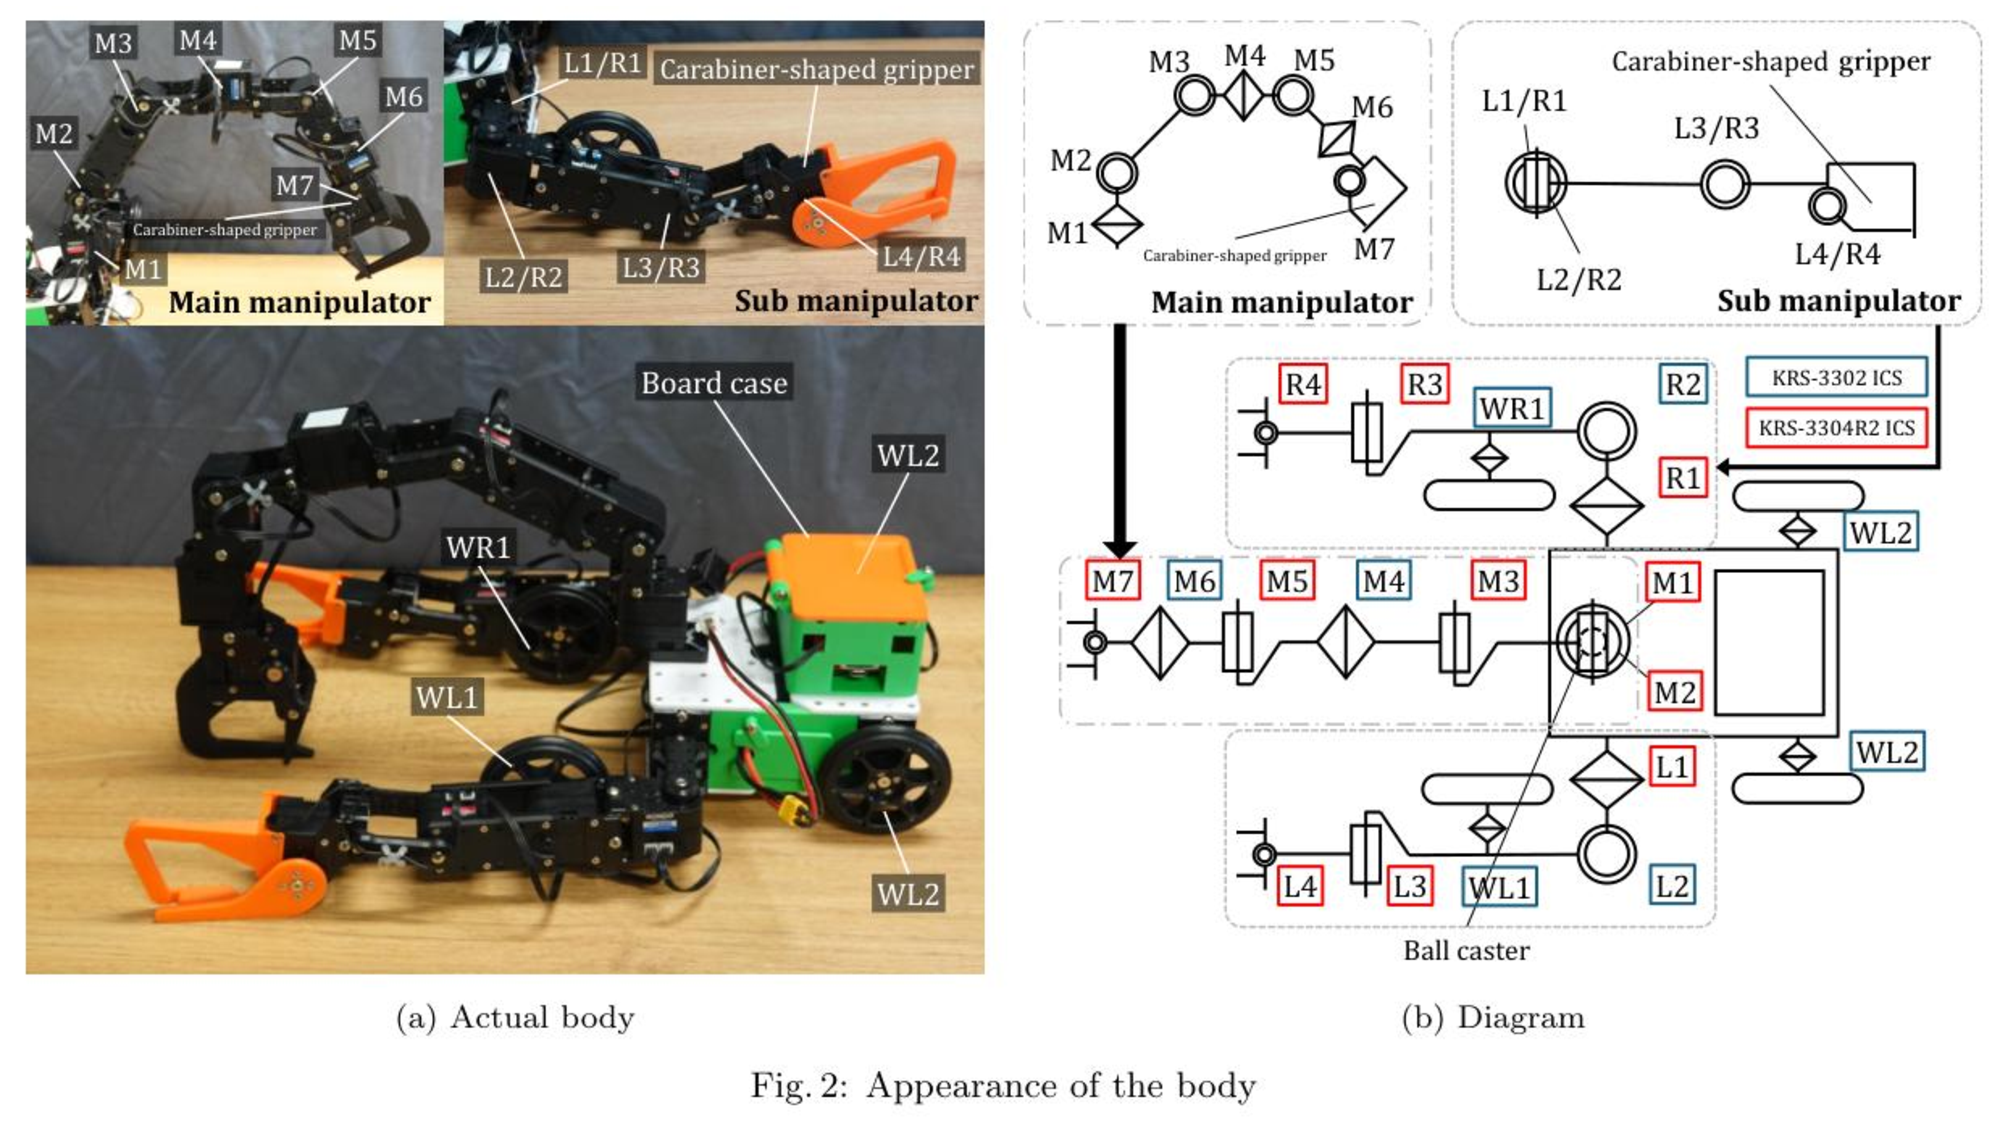
\includegraphics[width=.98\linewidth]{img/画像の集約_良い例.pdf}
    \subcaption{良い例}
  \end{minipage}
  \caption{画像は1つにまとめる}\label{fig:画像は1つにまとめる}
\end{figure}
%----------------------------------------------------------------------
\subsection{ダミー図の利用}
執筆と実験はだいたい同時並行で行われ,実験中に機体構成を一部変更したりすることがある.こういった理由から図に使う写真は最後にとりたい(特にKXR班).実験等で機体構成が確定するまでは図の部分を縦横比を揃えたダミーの図に置き換えておくことで後から撮った写真に置き換えられて楽.

%----------------------------------------------------------------------
\subsection{表の作成}\label{subsec:表の作成}
論文の表は表\ref{tab:net_info}のように縦線がないほうがかっこいい.
ただ,研究室の過去の論文やIEEEエクスプローラー等で出てくる論文を見るとわかるが,縦線がある表も普通にある.また,表はエクセルで作成して以下のサイトでtexの形式に変換するのが楽.

{\footnotesize \url{https://www.tablesgenerator.com/}}

\begin{table}[t]
  \centering
  \caption{Grid and string diameter of the nets used in the experiment and their general usage}
  \label{tab:net_info}
  \small
  \begin{tabular}{ccc}
    \hline
    Grid\,[$\si{mm}$] & String diameter\ [$\si{mm}$] & General use \\ \hline
    $25$ & $1.85$ & Golf net \\
    $35$ & $2.4$  & Baseball net \\ \hline
  \end{tabular}
  \vspace{-10mm}% どうしてもスペースを詰めたい場合や謎のスペースが入る場合はvspaceで詰める.
\end{table}

%----------------------------------------------------------------------------------------------------------
\section{bibtex}
引用を行うときはtexファイルの他にbibファイルを用意し,まとめておくことで,管理が楽になる.

論文を集める時はbibファイル用のデータも一緒に集めておくとよい.以下に各論文検索サイトでのbibデータの見方をまとめておく.
\begin{itemize}
  \item Google Scholar
  \begin{itemize}
    \item 検索画面 $>>$ 引用 $>>$ BibTex
  \end{itemize}
  \item IEEE Xplore
  \begin{itemize}
    \item 記事画面 $>>$ Cite This $>>$ BibTex
  \end{itemize}
  \item J-STAGE
  \begin{itemize}
    \item 記事画面 $>>$ BiB TEX形式
  \end{itemize}
\end{itemize}

上の方法で集めた場合,doi項目やurl項目が含まれているがいらないので消去する.

また,学会発表は上の方法だと出てこないので自分で作成する必要がある.ミスに注意.また,ページ番号の代わりに発表番号を書く.普通にpages項目に書くとpp.2B4-05のようにpp.がついてしまうため,note項目に発表番号,発表年の順に書くと\cite{cite:my_si}のように正しく出力される.
%----------------------------------------------------------------------------------------------------------
\section{項目の引用}\label{sec:ここは章}
項目の引用を行うときはラベルを定義する.例えば\ref{subsec:表の作成}節を引用したい場合,\verb|\label{subsec:表の作成}|でラベルを定義して,\verb|\ref{subsec:表の作成}|で引用する.このときラベルの命名法としては
\begin{quote}
  属性名:キャプション,見出し名
\end{quote}
とすることをお勧めする.

この方法は,ラベル名が推測しやすく,章の名前と図のキャプションで同じものがあっても特別なラベル名にしなくてよくなる.

\subsection{ここは節}\label{subsec:ここは節}
\subsubsection{ここは項}\label{subsubsec:ここは項}

また,見出しを引用するときは名前に注意する.それぞれ,\ref{sec:ここは章}章,\ref{subsec:ここは節}節,\ref{subsubsec:ここは項}項である.
%----------------------------------------------------------------------------------------------------------
\section{原稿の圧縮}
学会など提出できるpdfのサイズに制限がある場合,pdfの圧縮が必要.このとき,画像の解像度を下げる手法がよく使われるが,面倒.texのインストールで一緒にインストールされるghostscriptを使用する方法が楽.以下のコマンドをvscodeのターミナルで実行する.

{
  \small % ここからコピペ
  rungs -sDEVICE=pdfwrite -o output.pdf -dCompatibilityLevel='1.4' -dPDFSETTINGS=/ebook  -dNOPAUSE -dQUIET -dBATCH out/sample.pdf
}

なお,出力品質(-dPDFSETTINGS)は以下から選べる.

{
  \small % ここからコピペ
  /default,
  /screen,
  /ebook,
  /printer,
  /prepress,
}
%----------------------------------------------------------------------------------------------------------
\section{修正稿の提出}
原稿はslackの木村先生と工藤先生が一緒に入ったチャンネルに送る.このとき,工藤先生はpdfをタブレットで見るそうで,容量を数MBに圧縮してほしいらしい.

指摘点を修正し,修正稿を送るときは修正した点を\verb|\textcolor{red}{}|などで\textcolor{red}{赤く}しておくとわかりやすい.
また,修正の指示などで章を消したりするときは直接消さずコメントアウトで非表示にする.
%----------------------------------------------------------------------------------------------------------
\section{ショートカットの利用}
texのマクロには\verb|$$|や\verb|\mathrm|のように,よく使う割に打ちにくかったり長いものがある.このようなマクロはショートカットで呼び出せるようにしておくと時短になる.

本ファイルでは以下のショートカットを用意した.

\begin{tabular}{ll}
  @mr  & \verb|\mathrm{}|\\
  @mr2 & \verb|$\mathrm{}$|\\
  @equ & \verb|$$|\\
  @red & \verb|\textcolor{red}{}|\\
  @sl & section前の仕切り\\
  @sl\_s & subsection前の仕切り\\
  @sl\_ss & subsubsection前の仕切り
\end{tabular}

新たに作る場合は\verb|.vscode/settings.json|の以下の項目に書き加える.

{\small
\verb|"latex-workshop.intellisense.atSuggestion.user":|}
%----------------------------------------------------------------------------------------------------------
{\small
\bibliographystyle{jplain}
\bibliography{template}
}
\end{document}
